\addbibresource{reference.bib}

\chapter{Návrh architektury}\label{chap:arch}
V této kapitole bude čtenář seznámen s návrhem a koncepcí softwarového systému \textbf{Pixnet} - software pro distribuované řízení sítě částicových pixelových detektorů, který byl navržen a implementován v rámci této práce. V této kapitole bude popsána motivace pro vznik tohoto systému a budou představeny jednotlivé komponenty systému a jejich vzájemné interakce. Pro detailnější popis návrhu a implementace komponent viz kapitoly \ref{chap:handler}, \ref{chap:katherine} a \ref{chap:master}.

%********************************************************************************
% Motivace
%********************************************************************************
\section{Motivace}\label{chap:arch:motivation}
Hlavní motivací pro vznik tohoto systému je fakt, že moderní částicové pixelové detektory jsou schopné generovat vysoký datový tok, například \textit{Timepix3} má teoretické maximum \unit{5,12}{Gb/s} (viz \ref{chap:detectors:medipix_overview:timepix3}), takže nedistribuovaný systém, který by operoval na jedné instanci, by nebyl schopný zpracovat datový tok, který síť o vice detektorech je schopná generovat. 

Zde je možné namítnout, že každý systém je možné škálovat vertikálně\footnote{Škálováním v kontextu počítačových systému rozumíme změnu vlastností daného systému za účelem zvýšení, nebo snížení jeho výpočetního výkonu (ev. jiného sledovaného parametru). Zatímco u vertikálního škálování měníme vlastnosti jednoho uzlu systému (například přidáváním procesorů, pamětí, kapacity úložiště apod.), u horizontálního škálování přidáváme jednotlivé uzly - samostatné  jednotky (např. počítače). Pro úplnost je třeba doplnit že vertikální škálování má své omezení z hlediska použitého hardware, u horizontálního škálování žádná taková omezení nejsou.}. Zatímco cena škálování horizontálně škálovatelného systému je lineární závislost výpočetního výkonu na ceně, u vertikálně škálovatelného systému tato závislost roste exponenciálně. Jelikož vertikální škálování takového systému je  vysoce neefektivní, nebude dále uvažováno a tato práce se bude věnovat jenom návrhu a implementaci horizontálně škálovatelného řešení.

 Další motivací pro vytvoření tohoto systému je možnost řízení heterogenní sítě detektorů homogenním způsobem. Heterogenní sítí detektorů rozumíme takovou síť, ve které jsou detektory různých typů (například \textit{Timepix}, \textit{Timepix3} apod, viz \ref{chap:detectors:medipix_overview}), komunikující různými komunikačními protokoly prostřednictvím různých vyčítacích rozhraních (například \textit{Katherine}, \textit{ATLAS Pix} apod, viz \ref{chap:detectors:readouts}). V další části textu bude detailně popsána navržená a implementovaná modulová architektura, která výše zmíněné umožňuje.

 Pro potřeby experimentu \textit{ATLAS TPX} byl již vyvinut software \cite{atlastpx_sw,BegeraBcThesis2016} pro řízení sítě detektorů \textit{Timepix} \ref{chap:detectors:medipix_overview:timepix}, prostřednictvím vyčítacího rozhraní \textit{ATLAS Pix} \ref{chap:detectors:readouts:atlaspix}. Software však nevyhovuje požadavkům zmíněných výše:
 \begin{enumerate}[label=(\roman*)]
     \item \textbf{Škálovatelnost} - systém je navržen bez možnosti horizontálního škálování. Všechny detektory sítě jsou řízeny z jednoho uzlu a všechna vygenerovaná data jsou jím zpracovávány. Možnost použití pouze jednoho uzlu představuje nejslabší článek systému, který nemůže být použit pro řízení a vyčítání dat z větší sítě detektorů.
     \item \textbf{Modularita} - systém implementuje pouze komunikační protokol vyčítacího rozhraní \textit{ATLAS Pix} \ref{chap:detectors:readouts:atlaspix}. Přidání podpory nového vyčítacího rozhraní představuje významnou modifikaci architektury systému a pro nasazení nové verze je nutná odstávka celého systému.
 \end{enumerate}
Pro potřeby modernizace sítě \textit{ATLAS TPX} (za použití detektorů \textit{Timepix3}) bylo rozhodnuto o vývoji software, který bude navržen a implementován tak, aby požadavky na škálovatelnost a modularitu byly zohledněny.

%********************************************************************************
% Softwarová architektura
%********************************************************************************
\section{Softwarová architektura}\label{chap:arch:sw}
V této podkapitole budou popsány jednotlivé komponenty softwarové architektury systému Pixnet a bude vysvětlena jejich funkce. Na obrázku \ref{fig:arch:sw_architecture} jsou zobrazeny základní komponenty systému, včetně jejich kardinalit. Detektory sítě jsou řízeny handlery, které komunikují s detektory pomocí dodaného komunikačního protokolu (na obr. \ref{chap:arch:sw} jako \textit{komunikační interface}) a vyčítají z nich data, která jsou pak ukládána do datového úložiště (pomocí dodané implementace datového interface). Jednotlivé handlery jsou řízeny centrálním uzlem systému - masterem. Master je zodpovědný za konfiguraci systému, držení jeho stavu a přiřazování detektorů masterům.

\begin{figure}[h]
	\begin{center}
		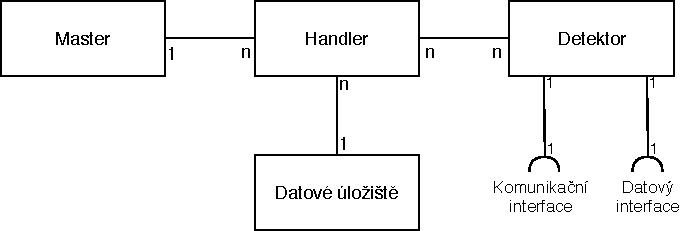
\includegraphics[width=14.5cm]{figures/arch_sw.pdf}
		\caption{Pixnet: softwarová architektura.}
		\label{fig:arch:sw_architecture}
	\end{center}
\end{figure}

V následujících podkapitolách budou detailněji popsány jednotlivé komponenty z obrázku~\ref{chap:arch:sw}.
\subsection{Detektor}\label{chap:arch:sw:detector}
Detektor je logická jednotka systému, která je reprezentována implementací komunikačního a datového interface, konfigurací a svým stavem. Fyzické propojení s detektorem je realizováno implementací komunikačního interface.

Komunikační interface obsahuje například metody pro navazování spojení s detektorem, metody pro nahrávání konfigurace a metody pro získání podporovaných příkazů detektoru a jejich vykonání. Každý příkaz má svoje ID, název a model vstupních a výstupních hodnot. Modelem hodnot rozumíme množinu parametrů různých datových typů (\texttt{boolean}, \texttt{integer}, \texttt{float} apod.), které můžou nabývat hodnot omezených zadaným intervalem, nebo jedné z předdefinovaných diskrétních hodnot.

Datový interface obsahuje kromě inicializačních metod (předání konfigurace detektoru apod.) také metodu pro předání reference na asynchronní frontu naměřených dat, do které jsou data vkládána implementací komunikačního interface. Datový interface může mít několik implementací - například data můžou být ukládána do datového úložiště handleru a následně asynchronně nahrána do centrálního datového úložiště, nebo můžou být rovnou synchronně nahrávána do datového úložiště.

\subsection{Datové úložiště}
Datové úložiště by mělo být škálovatelné, protože pro sítě o vetším počtu detektorů by ukládání dat do jednoho uzlu znamenalo omezení maximálního datového toku, dané kapacitou daného uzlu.

Jednou z možností implementace by mohlo být využití distribuovaného souborového systému, například \textit{Hadoop Distributed File System} \cite{HDFS}, který se v praxi\footnote{například v roce 2010 internetová společnost \textit{Yahoo!} používala \texttt{HDFS} pro persistenci \unit{25}{PB} podnikových dat \cite{HDFS}.} používá pro distribuované ukládání dat s možností jejich redundance na více uzlech (pro potřeby zálohování). 

Další možností může být použití nějaké \texttt{NoSQL} distribuované databáze, například \textit{MondoDB} (viz \ref{chap:arch:technologie:mongodb}).

\subsection{Handler}
Handler je komponenta, kterou je řízena podmnožina detektorů detektorové sítě. K jednomu handleru je tedy možné připojit $n$ detektorů, kde $n$ je omezeno sumou datového toku přes všechny připojené detektory v závislosti na maximálním možném datovém toku handleru.

Handler komunikuje s detektorem pomocí dodané implementace jeho komunikačního interface a data detektorem vygenerovaná jsou pomocí implementace datového interface uloženy do datového úložiště, nebo zpracovány jiným způsobem.

Handler je zodpovědný za zavedení dodaných implementací komunikačního a datového interface do systému. například po přiřazení detektoru handleru, handler získá seznam podporovaných příkazů detektoru a poskytne je masteru. To systému umožňuje řízení heterogenní sítě detektorům homogenním způsobem, jak již bylo zmíněno v \ref{chap:arch:motivation}.

Aby mylo možné handlery, potažmo detektory, řídit centralizovaně, handler poskytuje \texttt{API}\footnote{Z angl. \textit{Application programming interface} (aplikační programové rozhraní).}. Pomocí \texttt{API} jsou jednotlivé handlery připojovány do systému, handlerům jsou přiřazovány a odebírány detektory, inicializuje se konfigurace detektorů a ji řízena akvizice dat.

\subsection{Master}
Master je centrální prvek systému, jehož prostřednictvím jsou řízeny handlery. Master poskytuje \texttt{API} pro své řízení pomocí pomocí frontendové aplikace. Tato aplikace je webový tenký klient, který uživateli poskytuje uživatelské rozhraní pro řízení systému.

Když například uživatel přidává nový detektor do systému, tak nejprve skrze uživatelské rozhraní frontend aplikace zadá parametry detektoru, včetně implementace komunikačního a datového rozhraní, jak je znázorněno na obr. \ref{fig:arch:handler:new_detector}. Poté pomocí je detektor nahrán do mastera pomocí jeho \texttt{API}, kde je následně perzistentně uložen do jeho databáze. Při přiřazování detektoru handleru je konfigurace detektoru včetně implementace komunikačního a datového interface nahrána do zvoleného handleru, kde je dále zpracována. Zpracování konfigurace probíhá v následujících krocích:
\begin{enumerate}
    \item Vytvoření instance komunikačního interface a ověření jeho validity.
    \item Vytvoření instance datového interface a ověření jeho validity.
    \item Syntaktická analýza (tzv. \textit{parsing}) konfigurace detektoru a její nahrání do instancích komunikačního a datového interface.
    \item Vytvoření asynchronní fronty měřených dat a její předání instancím komunikačního a datového interface.
\end{enumerate}
Po dokončení inicializační sekvence je uživatel notifikován a v případě úspěšného dokončení je detektor připraven vykonávat příchozí příkazy a měřit data.

\begin{figure}[th!]
	\begin{center}
		\begin{sequencediagram}
            \newthread[blue_ligh]{mf}{Master frontend}
            \newinst[0.5]{mb}{Master backend}
            \newinst[0.5]{h}{Handler}
            \newinst[0.5]{d}{Detektor}
            \newinst[0.19]{c}{\shortstack{Impl kom.\\interface}}
            \newinst[0.19]{p}{\shortstack{Impl dat.\\interface}}
            
            % nahrání konfigurace
            \postlevel
            \begin{call}{mf}{
                %pro úpravu thread color
                %\tikzset{threadstyle/.style={top color=white,bottom color=red}}
                    \shortstack{
                        Přidání nového\\
                        detektoru
                    }
                }{mb}{výsledek}
                
                \begin{callself}{mb}{\shortstack{Validace a uložení\\konfigurace detektoru}}{výsledek}
                    \postlevel
                \end{callself}	
                
            \end{call}

            % binding
            \postlevel
            \postlevel
            \begin{call}{mf}{\shortstack{Přiřazení detektoru\\handleru}}{mb}{výsledek}
                
                \postlevel
                \begin{call}{mb}{\shortstack{Přiřazení\\detektoru}}{h}{výsledek}
                    
                    \begin{call}{h}{\shortstack{Inicializace}}{d}{výsledek}
                        
                        \begin{call}{d}{\shortstack{Inicializace\\(konfig.,\\fronta dat)}}{c}{}
                        \end{call}
                        
                        \postlevel
                        \postlevel
                        \begin{call}{d}{\shortstack{Inicializace\\(konfig., fronta dat)}}{p}{}
                        \end{call}

                        %\begin{call}{d}{\shortstack{Zavedení\\modulu}}{c}{}
                        %\end{call}
    
                        %\begin{call}{d}{\shortstack{Zavedení modulu}}{p}{}
                        %\end{call}

                        %\postlevel
                        %\begin{call}{d}{\shortstack{Nahrání\\konfigurace}}{c}{}
                        %\end{call}

                        %\begin{call}{d}{\shortstack{Nahrání konfigurace}}{p}{}
                        %\end{call}
        
                        %\begin{messcall}{d}{\shortstack{Fronta dat}}{c}
                        %\end{messcall}

                        %\begin{messcall}{d}{\shortstack{Fronta dat}}{p}
                        %\end{messcall}
        
                    \end{call}
        
                \end{call}

            \end{call}
            
		\end{sequencediagram}
		\caption{Sekvenční diagram znázorňující příklad přidání detektoru do systému a jeho přiřazení handleru.}
		\label{fig:arch:handler:new_detector}
	\end{center}
\end{figure}

Jako datové úložiště pro konfigurace detektorů, informace o jejich stavu a o stavu jednotlivých handlerů bude navržena relační \texttt{SQL}\footnote{Z angl. \textit{Structured Query Language} (strukturovaný dotazovací jazyk).} databáze, ke které bude přistupovat pouze backend mastera.

%********************************************************************************
% Hardwarová architektura
%********************************************************************************
\section{Hardwarová architektura}
V předchozí podkapitole byla popsána softwarová architektura. Fyzická instalace sítě přináší další omezení, především z pohledu síťové infrastruktury, které budou popsány v této podkapitole.

Na obrázku \ref{fig:arch:hw_architecture} je příklad sítě sestávající se ze dvou podsítí (tzv. \textit{subnetwork}). Podsítí rozumíme takovou podmnožinu detektorů a handlerů, ve které libovolný detektor může být přiřazen libovolnému handleru. Pro úplnost je třeba doplnit, že nutnou podmínkou je, aby všechny handlery měly spojení s masterem a s distribuovaným úložištěm naměřených dat.

\begin{figure}[h]
	\begin{center}
		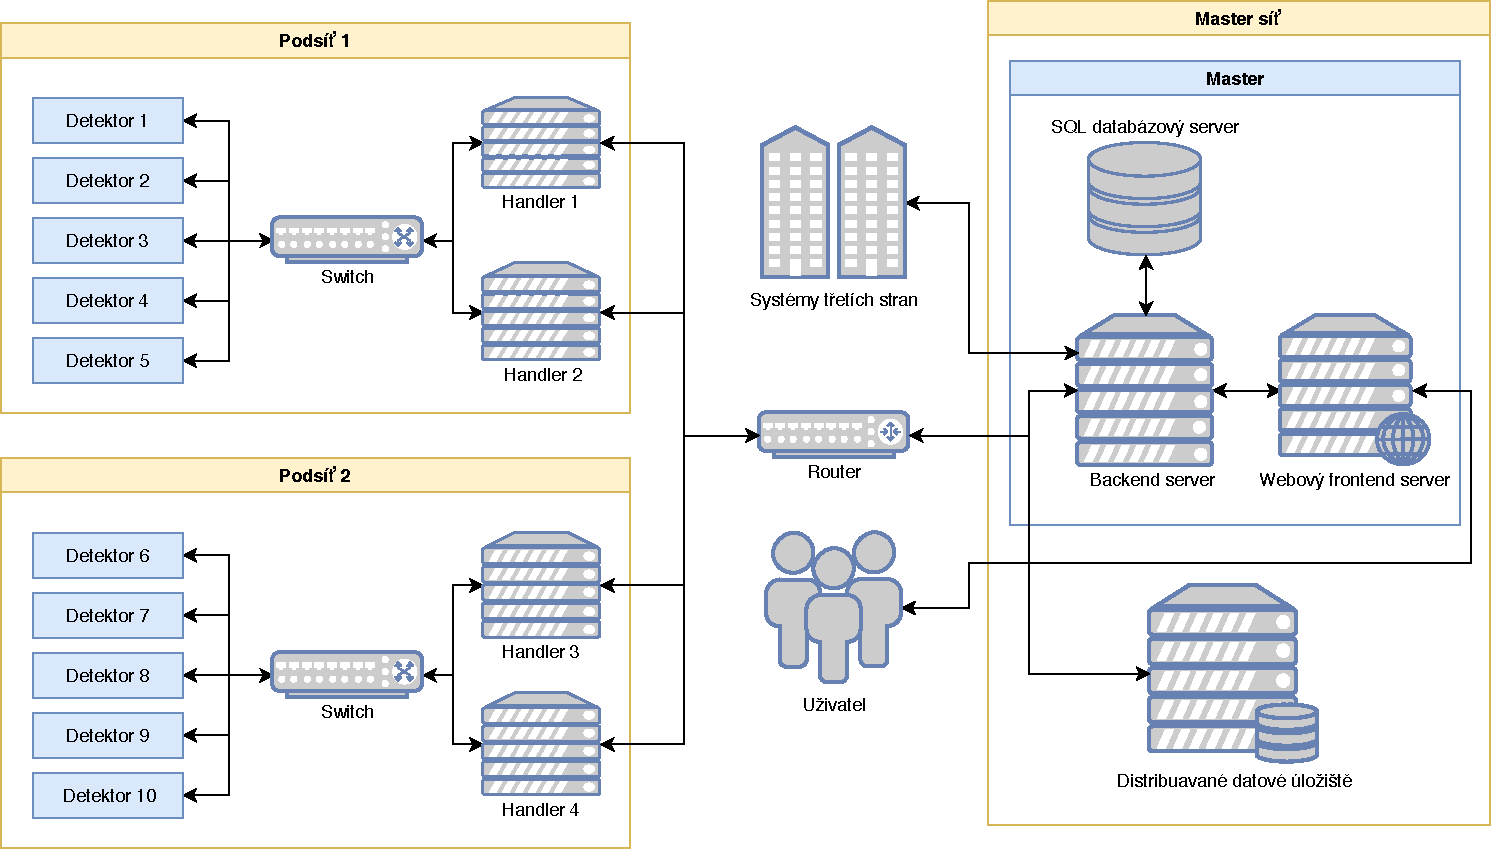
\includegraphics[width=15cm]{figures/arch_hw.pdf}
		\caption{Pixnet: hardwarová architektura s příkladem realizace sítě o dvou podsítích, kde v každé jsou dva handlery a pět detektorů, mastera (s \textit{SQL} databází pro persistenci konfigurace a frontend server poskytující webovou aplikaci) a centrálního datového úložiště naměřených dat.}
		\label{fig:arch:hw_architecture}
	\end{center}
\end{figure}

Master se skládá ze tří komponent:
\begin{description}
    \item[Backend serveru] implementujícího business logiku pro komunikaci s handlery (jako například přiřazování detektorů, řízení akvizice dat apod.). Server zároveň poskytuje \textit{API} pro možnou integraci s webovým frontend serverem se systémy třetích stran\footnote{Například pro experiment \textit{ATLAS TPX} v CERN je plánována integrace s \texttt{DAC} \cite{cern_dcs} (\textit{Detector control system}), který umožňuje centrální řízení detektorových systému, včetně integrace do bezpečnostního systému \texttt{DSS} (\textit{Detector safety system}), datového akvizičního systému \texttt{DAQ} (\textit{Data Acquisition System}) apod.}, kterými muže být plnohodnotně řízen.
    \item[Databázového serveru] poskytující relační \texttt{SQL} databázi pro persistenci konfigurace systému, včetně implementace potřebných rozhraní, stavových informací sítě apod.
    \item[Frontend serveru] poskytujícího webovou aplikaci s uživatelským rozhraním pro řízení mastera pomocí jeho \texttt{API}, resp. pro řízení celé sítě.
\end{description}

Na příkladu zmíněném výše je sít využívající jedno centrální datové úložiště. Realizace této komponenty je závislá na poskytnuté implementaci datových rozhraní jednotlivých detektorů. Může být implementovaná pomocí centralizovaného, nebo distribuovaného systému. Umístění úložiště také není omezeno - může být umístěno v sítě mastera, v jednotlivých podsítích, v síti mastera i v jednotlivých podsítích (buffer pro malou šířku pásma spojení podsíť - master síť), nebo třeba v internetu (cloudové úložiště, jako například \textit{Firebase Firestore}, \textit{Amazon 3S}, \textit{Microsoft Azure} apod.).

%********************************************************************************
% Škálovatelnost
%********************************************************************************
\section{Škálovatelnost}
Škálování systému Pixnet je teoreticky neomezeno. Kritickým bodem každého datového akvizičního systému je vyčítání a ukládání naměřených dat. Tento problém je řešen horizontálním škálováním, spočívajícím v přidáváním handlerů, které zajišťují komunikaci s detektory a ukládání naměřených dat.

Možnost škálování datového úložiště je závislá na instanci hardwarové architektury popsané výše. V \cite{gandini2014performance} bylo ukázáno, že \texttt{NoSQL} databázové systémy (jako například \textit{MongoDB} nebo \textit{Apache Cassandra}) jsou dobře horizontálně škálovatelné a jsou schopny zajistit dostatečnou rychlost zápisu vstupních dat. Takže například pro instanci sítě s vhodně zvoleným distribuovaným datovým úložištěm, umístěným v síti mastera (viz obr. \ref{fig:arch:hw_architecture}), budou požadavky na persistenci naměřených dat splněny.

%********************************************************************************
% Toužité technologie
%********************************************************************************
\section{Použité technologie}\label{chap:arch:technologie}
V této podkapitole budou stručně shrnuty technologie použité při implementaci systému.

\begin{description}
    \item[Java] je staticky typovaný, objektově orientovaný programovací jazyk a byl při zahájení implementace zvolej jako primární programovací jazyk pro vývoj tohoto systému. Byl zvolen především díky své jednoduchosti, výkonosti a přenositelnosti. 
    
    Java je interpretovaný programovací jazyk - při kompilaci kód není kompilovaný do strojového kódu zvolené platformy, ale do tzv. \textit{bytecode}, který je platformně nezávislý. \textit{Bytecode} pak může být spuštěn na libovolném počítači či zařízení, které disponuje interpretem Javy - \texttt{JVM} (\textit{Java Virtual Machine}). Java není čitě interpretovaný programovací jazyk, protože v pozdějších verzích byla přidána podpora pro \texttt{JIT} (tzv. \textit{Just-in-time}) kompilátoru, který umožňuje dynamickou kompilaci \textit{bytecode} do strojového kódu dané platformy, díky čemuž můžu Java ve srovnání s neinterpretovaný
    my programovacími jazyky (\texttt{C++} apod.) dosahovat srovnatelných výsledků.
    
    Java také obsahuje nástroj pro generační správu paměti (tzv. \textit{Garbage Collector}), který se stará o automatické uvolňování paměti mazáním objektů, na které neukazuje žádná reference. Tento nástroj je pro dlouhodobě běžící serverové systémy velice užitečný.

    \item[Kotlin]\label{chap:arch:technologie:kotlin} je moderní staticky typovaný, objektově orientovaný programovací jazyk, který běží nad \texttt{JVM}. Hlavní výhoda Kotlinu je jeho interoperabilita - kód může být zkompilovaný do Java \textit{bytecode}, do JavaScriptu, nebo i do nativního kódu s tím, že může používat závislosti dané platformy (například pro kompilaci do Java \textit{bytecode} může používat Java knihovny, takže část kompilovaného kódu může být napsána v Javě a část v Kotlinu).

    Oproti Javě poskytuje mnoho výhod, jako například \textit{null-safety} (každá proměnná má kromě svého datového typu i příznak, jestli může být \texttt{null}, což eliminuje spoustu chyb, se kterými se můžeme setkat například v Javě), podpora funkcionálního stylu programování (oproti javě může být v proměnné uložená funkce), \textit{extension functions} (podobně jako v \texttt{C\#}, je možné přidat funkci do dané třídy bez nutnosti její modifikace, nebo vytvořené poděděné třídy) a další vylepšení. 
    
    Především díky výhodám popsaným výše, bylo v pozdější fázi vývoje rozhodnuto o použití Kotlinu, coby primárního programovacího jazyku pro handler a backend mastera. Také bylo experimentování s použitím Kotlinu pro frontend mastera, pomocí vytvoření společné \textit{code-base} pro backend a frontend mastera (sestávajícího se z business logiky a modelu), ale od tohoto přístupu bylo upuštěno z důvodů omezené podpory kompilátoru Kotlin kódu do JavaScriptu a z důvodu omezené komunitní podpory.
    
    \item[JavaScript] je interpretovaný, objektově orientovaný programovací jazyk, který je zpravidla používán pro tvorbu webových aplikací, ale má i jiné aplikace. V kontextu webových aplikací, JavaScript kód je interpretován na klientské straně v prohlížeči a pomocí jeho \textit{API} manipuluje s načtenou HTML stránkou, resp. její vnitřní interpretací webovým prohlížečem - tzv. \texttt{DOM} (\textit{Document Object Model}).
    
    V rámci této práce je použit pro implementaci frontendové části mastera - webové aplikace poskytující uživatelské rozhraní pro obsluhu systému Pixnet.
     
    \item[Gradle] Je automatizovaný build\footnote{Sestavování počítačových programů.} systém, který vychází z \textit{Apache Ant} a \textit{Apache Maven} a používá \texttt{DSL}\footnote{Z angl. \textit{domain-specific language} (doménově specifický jazyk)} založeném na \textit{Groovy} a \textit{Kotlin}. Umožňuje automatizované stahování a správu závislostí a knihoven z online repositářů (kromě \textit{Gradle} i \textit{Maven} a \textit{Ivy} pro kompatibilitu s dalšími build systémy).
    
    \item[Spring]\label{chap:arch:technologie:spring} je aplikační framework pro vývoj \texttt{J2EE}\footnote{Označení pro Java \textit{Enterprise Edition} - platformy pro vývoj podnikových systémů, odvozené od JavaSE (Standard Edition)} aplikací a v rámci systému Pixnet bude použit v rámci implementace handlera a mastera. Spring framework je sada modulů, které nabízejí nástroje jako například webový controller (pro poskytování \texttt{REST API}), \textit{Dependency Injection}\footnote{Technika pro vkládání závislostí mezi komponentami počítačového programu, aniž by v době kompilace měly komponenty na sebe referenci.}, JPA (\textit{Java Persistent API} pro práci s databází), podporu testování apod.

    Novější alternativou je Spring Boot, který je nadstavbou nad původním Spring frameworkem. Spring Boot odstraňuje nutnost komplikovaného definování konfigurace a také přináší možnost zapouzdření do samostatně spustitelné aplikace s embedovaným webovým serverem (\textit{Tomcat}, nebo \textit{Jetty}), takže již není třeba nasazovat \texttt{WAR}\footnote{Z angl. \textit{Web Application Archive} (archív se zkompilovanou webovou \texttt{J2EE} aplikací).} na webový server, protože Spring Boot aplikace je zkompilovatelná do spustitelné \texttt{JAR}\footnote{Z angl. \textit{Java Archive} (archív se zkompilovanou Java aplikací).} aplikace.
    
    \item[ReactJS] je JavaScriptová knihovna pro vývoj uživatelského rozhraní webových aplikací, vyvíjená společností Facebook. React je používán k vývoji tzv. \textit{single-page} aplikací, tj. takových webových aplikací, které k interakci s uživatelem používají jen jednu stránku, jejíž obsah dynamicky přepisují (na rozdíl od stahování nové stránky z webového serveru).
    
    React je založen na principu zapouzdřených komponent, kde každá komponenta ma svoje vlastnosti a svůj stav. Komponenty jsou znovupoužitelné a zanořitelné do jiných komponent. Navíc komponenty nepracují přímo s DOM prohlížeče, ale přistupují pouze k jeho virtuální reprezentaci, což umožňuje optimalizovat operace s DOM. Například když nějaká komponenta změní svůj stav (ev. tranzitivně i stav jiných komponent), tak se na stránce přegenerují jen takové komponenty, jejichž stav byl změněn.

    React bude použit pro implementaci frontendové webové aplikace mastera. Vedle Reactu existuje ještě React Native, který je určen pro hybridní vývoj mobilních aplikací, tím se ale v této práci nebudeme zabývat.
    
    \item[PostgreSQL] je nejpoužívanější open source objektově-relační databázový systém. Oproti klasickým relačním databázím (například \textit{MySQL}) má objektově orientovaný databázový model, který je přímo podporován databázovým schématem a dotazovacím jazykem.
    
    Tento databázový systém bude použit pro persistenci konfigurace sítě a bude k němu přistupovat backend mastera.
    
    \item[MongoDB]\label{chap:arch:technologie:mongodb} je \texttt{NoSQL} dokumentový databázový systém. Oproti tradičním relačním databázovým systémům jsou data ukládána do \texttt{BSON}\footnote{Binární forma JSON (z ang. JavaScript Object Notation)} dokumentů. Mezi hlavní výhody \textit{MondoDB} patří:

    \begin{description}
        \item[Indexace:] Na každé pole objektů v dokumentu lze vytvořit index a tím zrychlit vyhledávání v datech.
        \item[Replikace:] \textit{MondoDB} ukládá data do tzv. \textit{replica set}, která obsahuje jednu, nebo více replik dat. Pro případ více replik, jedna vždy funguje jako primární a ostatní jako sekundární, do kterých jsou replikována data z primární repliky. Hlavní výhoda spočívá ve vyšší dostupnosti dat (data lze číst z více replik současně) a spolehlivosti (když jedna replika selže, je nahrazena replikou jinou).
        \item[Horizontální škálování:] \textit{MondoDB} má podporu pro horizontální škálování pomocí tzv. \textit{shardingu} \cite{mongodb-scale}. \textit{Sharded cluster} je pak množina uzlů s jednotlivými \textit{shardy}, kde každý obsahuje podmnožinu \textit{shardovaných} dat.
    \end{description}

\end{description}